\documentclass[tikz,border=2pt]{standalone}
\usepackage{amsmath}
\usetikzlibrary{decorations.pathreplacing}
\begin{document}
% Area model of 3(4+5) = 3*4 + 3*5 = 12 + 15 = 27: a 3-by-(4+5) rectangle splits into a 3-by-4
% and a 3-by-5 rectangle.
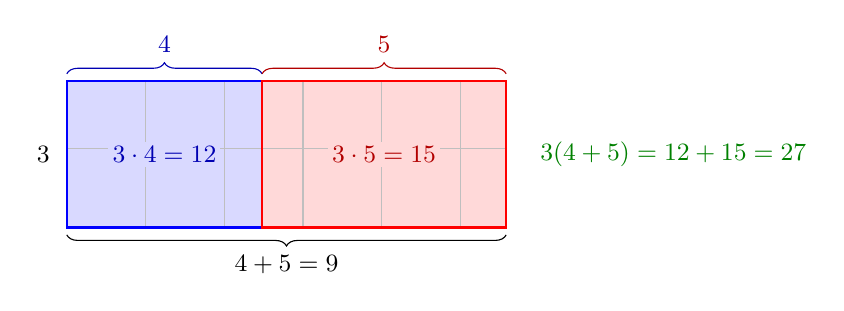
\begin{tikzpicture}[font=\small, x=0.62cm, y=0.62cm]
  \fill[blue!15] (0,0) rectangle (4,3);
  \fill[red!15] (4,0) rectangle (9,3);
  \draw[gray!50, thin] (0,0) grid (9,3);
  \draw[blue, thick] (0,0) rectangle (4,3);
  \draw[red, thick] (4,0) rectangle (9,3);
  \node[blue!70!black, fill=blue!15, inner sep=1.5pt] at (2,1.5) {$3\cdot4=12$};
  \node[red!70!black, fill=red!15, inner sep=1.5pt] at (6.5,1.5) {$3\cdot5=15$};
  % side lengths
  \node[anchor=east] at (-0.15,1.5) {$3$};
  \draw[decorate, decoration={brace, amplitude=4pt}, blue!70!black] (0,3.15) -- node[above=4pt] {$4$} (4,3.15);
  \draw[decorate, decoration={brace, amplitude=4pt}, red!70!black] (4,3.15) -- node[above=4pt] {$5$} (9,3.15);
  \draw[decorate, decoration={brace, amplitude=4pt, mirror}] (0,-0.15) -- node[below=4pt] {$4+5=9$} (9,-0.15);
  \node[green!50!black, anchor=west] at (9.5,1.5) {$3(4+5)=12+15=27$};
\end{tikzpicture}
\end{document}
